\documentclass[a4paper,11pt]{article}
\pdfoutput=1
%\usepackage{jheppub}
\usepackage{graphicx}% Include figure files
\usepackage{graphics}
\usepackage{dcolumn}% Align table columns on decimal point
\usepackage{bm}% bold math
\usepackage{epstopdf}
\usepackage{mathrsfs}
\usepackage{amssymb}
\usepackage{amsmath}
%\usepackage[pdftex]{hyperref}
%\usepackage{natbib}
\usepackage{multirow,cite}

\bibliographystyle{JHEP}

\def\bs{\boldsymbol}
\def\del{\partial}

%\def\p{{\boldsymbol p}_{\perp }}
%\def\pb{\bar {\boldsymbol p}_{\perp }}
%\def\pp{{\boldsymbol p}_{\perp }}
\def\p{{\boldsymbol p}}
\def\pb{\bar {\boldsymbol p}}
\def\pp{{\boldsymbol p}}
%\def\q{{\boldsymbol q}_\perp}
\def\q{{\boldsymbol q}}
\def\l{{\boldsymbol l}_\perp}
%\def\k{{\boldsymbol k}_\perp}
\def\k{{\boldsymbol k}}
\def\m{{\boldsymbol m}_\perp}
%\def\x{{\boldsymbol x}_\perp}
\def\x{{\boldsymbol x}}
\def\y{{\boldsymbol y}_\perp}
\def\X{{\boldsymbol X}_\perp}
\def\Y{{\boldsymbol Y}_\perp}
\def\D{{\boldsymbol D}_\perp}
\def\r{{\boldsymbol r}_\perp}
\def\z{{\boldsymbol z}_\perp}
%\def\v{{\boldsymbol v}_\perp}
\def\v{{\boldsymbol v}}
\def\w{{\boldsymbol w}_\perp}
\def\b{{\boldsymbol b}_\perp}
\def\Q{{\boldsymbol Q}_\perp}
\def\M{{\boldsymbol M}_\perp}
%\def\bkappa{{\boldsymbol \kappa}_\perp}
%\def\bbkappa{\bar{\boldsymbol \kappa}_\perp}
\def\bkappa{{\boldsymbol \kappa}}
\def\bbkappa{\bar{\boldsymbol \kappa}}
\def\bnu{{\boldsymbol \nu}_\perp}
\def\V{\hat{\boldsymbol v}_{1\perp}}
\def\K{\hat{\boldsymbol k}_{1\perp}}
\def\bV{\hat{\boldsymbol v}_{2\perp}}
\def\bK{\hat{\boldsymbol k}_{2\perp}}
\def\qqb{{q\bar q}}
\def\sM{{\scriptscriptstyle M}}

\newcommand{\beq}{\begin{eqnarray}}
\newcommand{\eeq}{\end{eqnarray}}
\newcommand{\be}{\begin{equation}}
\newcommand{\ee}{\end{equation}}
\newcommand{\nn}{\nonumber\\ }
\newcommand{\labe}{\label}
\newcommand{\bea}{\begin{eqnarray}}
\newcommand{\eea}{\end{eqnarray}}


\newcommand{\la}{\left\langle}
\newcommand{\ra}{\right\rangle}
\newcommand{\lc}{\left[}
\newcommand{\rc}{\right]}
\newcommand{\lp}{\left(}
\newcommand{\rp}{\right)}

%\bibliographystyle{JHEP}

%\textwidth=15.0cm \textheight=23.5cm
\textwidth=16.0cm \textheight=23.0cm 
\topmargin 0cm \oddsidemargin 0cm 
\setlength{\unitlength}{1mm}

\usepackage{url}
\usepackage{hyperref}

\begin{document}

\begin{center}
  {\Large \bf Extracting the Higgs self-coupling at a 100 TeV\\[0.2cm] hadron
  collider in the $b\bar{b}b\bar{b}$ final state}
\vspace{.7cm}

J. Katharina Behr, Daniela Bortoletto, James A. Frost,\\
  Nathan P. Hartland, Cigdem Issever and Juan Rojo


\vspace{.3cm}
{\it Physics Department, 1 Keble Road, University of Oxford, United Kingdom }

\end{center}
\vspace{1cm}


\paragraph{Introduction}

In this contribution, we provide a first estimate of the accuracy
in the Higgs self-coupling that can be achieved at a 100 TeV
hadron collider in the  $b\bar{b}b\bar{b}$ final state.
%
The analysis methodology is based on our recent feasibility
study~\cite{Behr:2015oqq}
for 14 TeV, with suitable modifications for the case of 100 TeV,
as we discuss below.
%
 Our strategy is based upon a combination of traditional cut-based
 methods and multivariate analysis (MVA).
  %
  We account for  all relevant
  backgrounds, including the contribution from mis-identified
  light and charm jets.
  %
  We also assess the robustness of our analysis strategy in
  an environment with high pileup (PU).
  %
 Our results indicate that 
  the $b\bar{b}b\bar{b}$ 
final state
alone should allow for the observation of double Higgs production
  at the HL-LHC.
  %
  We now discuss how our findings apply to the case of a 100
  TeV collider.
  %
  We note that other studies of Higgs pair production in this
final state can be found in Refs.~\cite{Wardrope:2014kya,deLima:2014dta}.

\paragraph{Monte Carlo sampling generation}


Higgs pair production is simulated at leading order (LO) using
{\tt MadGraph5\_aMC@NLO}~\cite{Alwall:2014hca}.
%
We use a tailored  model~\cite{Maltoni:2014eza}
for gluon-fusion Higgs boson pair production
which includes mass effects
from the
exact form factors for the top-quark triangle and box
loops~\cite{Plehn:1996wb}.
%
The calculation is performed in the
$n_f$=4 scheme,  accounting for  $b$-quark mass effects. 
The renormalization and factorization
scales are taken to be $\mu_F=\mu_R=H_T/2$.
%
For the input parton distribution functions (PDFs) we 
adopt the NNPDF 3.0 $n_f=4$ LO set~\cite{Ball:2014uwa} with
$\alpha_s(m_Z^2)=0.118$,
interfaced via {\tt LHAPDF6}~\cite{Buckley:2014ana}.
%
The Higgs boson couplings
and branching ratios are set to their SM values,
and its mass is taken to be
$m_h=125$ GeV~\cite{Aad:2014aba,Khachatryan:2014jba,Aad:2015zhl}.
%
To achieve the correct higher-order value of the
integrated cross-section, we rescale our LO signal sample to match the
NNLO+NNLL
inclusive calculation~\cite{deFlorian:2013jea,deFlorian:2015moa}.
%
Parton level signal events are then showered with the {\tt Pythia8} Monte
Carlo~\cite{Sjostrand:2007gs,Sjostrand:2014zea}, version {\tt v8.201},
using the  Monash 2013 tune~\cite{Skands:2014pea},
based on the NNPDF2.3LO PDF set~\cite{Ball:2012cx,Ball:2013hta}.
%
Background samples are generated at leading order
with {\tt SHERPA}~\cite{Gleisberg:2008ta} {\tt v2.1.1}.
%
As in the case of the signal generation,
the NNPDF 3.0 $n_f = 4$ LO set with strong coupling
$\alpha_s(m_Z^2)=0.118$ is used for all samples, and
we use as
factorisation and renormalisation scales $\mu_F=\mu_R=H_T/2$.
%
We account for all relevant background
processes that can mimic the
 $hh\to 4b$ signal process.
%
This includes  QCD $4b$ multi-jet production, as well as
QCD $2b2j$ and $4j$ production, and top quark pair
production.
%
Single Higgs production processes such as $Z(\to b\bar{b})h(\to b\bar{b})$
and $t\bar{t}h(\to b\bar{b})$ along with electroweak backgrounds e.g $Z(\to b\bar{b})b\bar{b}$,
are much smaller than the QCD backgrounds~\cite{Wardrope:2014kya,deLima:2014dta}
and are therefore not included in the present analysis.
%
The LO cross-sections for
the background samples have been rescaled so that the integrated
distributions reproduce known higher-order QCD results.
%
We take into account the finite energy and angular resolution of 
hadronic calorimeters.

\paragraph{Analysis strategy.}
After the parton shower, final state particles
are clustered using the
jet reconstruction algorithms
of
{\tt FastJet}~\cite{Cacciari:2011ma,Cacciari:2005hq},
{\tt v3.1.0}.
%
We use the following jet definitions:
\begin{itemize}
\item {\it Small-$R$ jets}, reconstructed with the
  anti-$k_T$ algorithm~\cite{Cacciari:2008gp} with $R=0.4$ radius.
  %
  Small-$R$ jets are required
  to have transverse momentum $p_T \ge 40$~GeV
  and pseudo-rapidity $|\eta|<2.5$, 

\item {\it Large-$R$ jets},  reconstructed with 
  anti-$k_T$ with $R=1.0$.
  %
  These are required to have
  $p_T \ge 200$~GeV, lie in the
  $|\eta|<2.0$ region and
  satisfy the  BDRS mass-drop tagger (MDT)~\cite{Butterworth:2008iy}.
    
\item {\it Small-$R$ subjets}, constructed by 
  by clustering all final-state particles with
 anti-$k_T$ with  $R=0.3$, that are then
 ghost-associated  to the large-$R$ jets~\cite{Aad:2015uka}.
 %
 They
  are required to satisfy
  $p_T > 50$~GeV and $|\eta|<2.5$.
\end{itemize}

For the   boosted and intermediate categories,
which involve large-$R$ jets,
we use a number of jet substructure variables~\cite{Salam:2009jx,Aad:2013gja}:
the $k_T$-splitting scale~\cite{Butterworth:2002tt,Butterworth:2008iy}, the ratio of 2-to-1 subjettiness $\tau_{21}$~\cite{Thaler:2010tr,Thaler:2011gf}, and the ratios of energy correlation functions (ECFs)  $C^{(\beta)}_2$~\cite{Larkoski:2013eya} and
$D_2^{(\beta)}$~\cite{Larkoski:2014gra}.
%
For each jet definition described above, a different
$b$-tagging strategy is adopted:

\begin{itemize}

\item {\it Small-$R$ jets}. If a small-$R$ jet has at least one $b$-quark among their constituents,
  it will be tagged as a $b$-jet with probability $f_b$.
  %
  In order to be considered in the $b$-tagging algorithm,
  $b$-quarks inside the small-$R$ jet
  should satisfy $p_T \ge 15$ GeV~\cite{Aad:2015ydr}.
  %
  The probability of tagging a jet is not modified
  if more than one $b$-quark is found among the jet constituents.
  %  
  If no $b$-quarks are found among the constituents
  of this jet, it can be still be tagged as a $b$-jet with
  a mistag rate of $f_l$, unless a charm quark is present instead,
  and in this case the mistag rate is $f_c$.
  %
  Only jets that contain at least one (light or charm)
  constituent
  with $p_T \ge 15$ GeV can induce a fake $b$-tag.
  %
  
  \item {\it Large-$R$ jets}. Large-$R$ jets are $b$-tagged by
    ghost-associating anti-$k_T$ $R=0.3$ (AKT03)
    subjets to the original large-$R$
    jets~\cite{Cacciari:2007fd,Aad:2013gja,
      ATLAS-CONF-2014-004,Aad:2015uka}.
    %
    A large-$R$ jet is considered $b$-tagged if both
    the leading and subleading AKT03 subjets, where the ordering
    is done in the subjet $p_T$, are both individually $b$-tagged,
    with the same criteria as the small-$R$ jets.
    %
     Therefore, a large-$R$ jet where the two leading
    subjets have at least one $b$-quark will be tagged
    with probability $f_b^2$.
    %
    As in the case
    of small-$R$ jets, we only attempt to $b$-tag the two leading subjets,
    else one finds a degradation of the
    signal significance.
    %
    The treatment of the $b$-jet mis-identification
    from light and charm jets
    is the same as for the small-$R$ jets.
  
\end{itemize}

For the $b$-tagging probability $f_b$, along with
the $b$-mistag probability of light ($f_l$) and charm ($f_c$) jets,
we use the values $f_b=0.8$, $f_l=0.01$
and  $f_c=0.1$.
%The s
Our analysis strategy follows the
scale-invariant resonance tagging of Ref.~\cite{Gouzevitch:2013qca}.
%
Rather than restricting to a specific event topology,
we consistently combine the information from
the three possible topologies: boosted, intermediate and
resolved, with the optimal cuts for each category being determined
separately.
%
The three categories are defined as follows:
\begin{itemize}
\item {\it Boosted category}. An event which
  contains at least two large-$R$ jets, with the two leading jets
 being $b$-tagged.
\item {\it Intermediate category}. An event with exactly one  $b$-tagged, large-$R$ jet, which
  is assigned to be the leading Higgs candidate.
  %
  In addition, we require at least two $b$-tagged, small-$R$ jets,
  which must be separated with respect to the large-$R$ jet
  by  $\Delta R\ge 1.2$.
  %
    
\item {\it Resolved category}. An event with at least
  four $b$-tagged small-$R$ jets.
  %
  The two Higgs candidates are reconstructed out of the
  leading four small-$R$ jets in the event by minimizing the relative difference of
  dijet masses.
  %
  
\end{itemize}
Once a Higgs boson candidate has been identified,
its invariant mass is required to lie within a fixed window
of width $80~{\rm GeV}$ around the nominal Higgs boson mass of $m_h= 125$
GeV.
%

\paragraph{Results.} We now discuss the results of our analysis
at the end of the MVA.
%
First we discuss the statistical significance of a measurements
of the $hh\to 4b$ cross-section at 100 TeV and then provide
a first estimate on the accuracy of the extraction of the self-coupling.
%
The specific type of  MVA that we use to
disentangle signal and background events is
a multi-layer feed-forward artificial neural network (ANN),
known as a {\it perceptron}.
%
This family of ANNs are also known as {\it deep neural networks},
due to their multi-layered architecture.
%
The MVA inputs are a set of kinematic variables describing the
signal and background
events which satisfy the requirements of the
cut-based analysis.
%
The output of the trained ANNs also allows for the identification,
in a fully automated way,
of the most relevant variables in the discrimination between 
signal and background.


%%%%%%%%%%%%%%%%%%%%%%%%
\begin{figure}[t]
\begin{center}
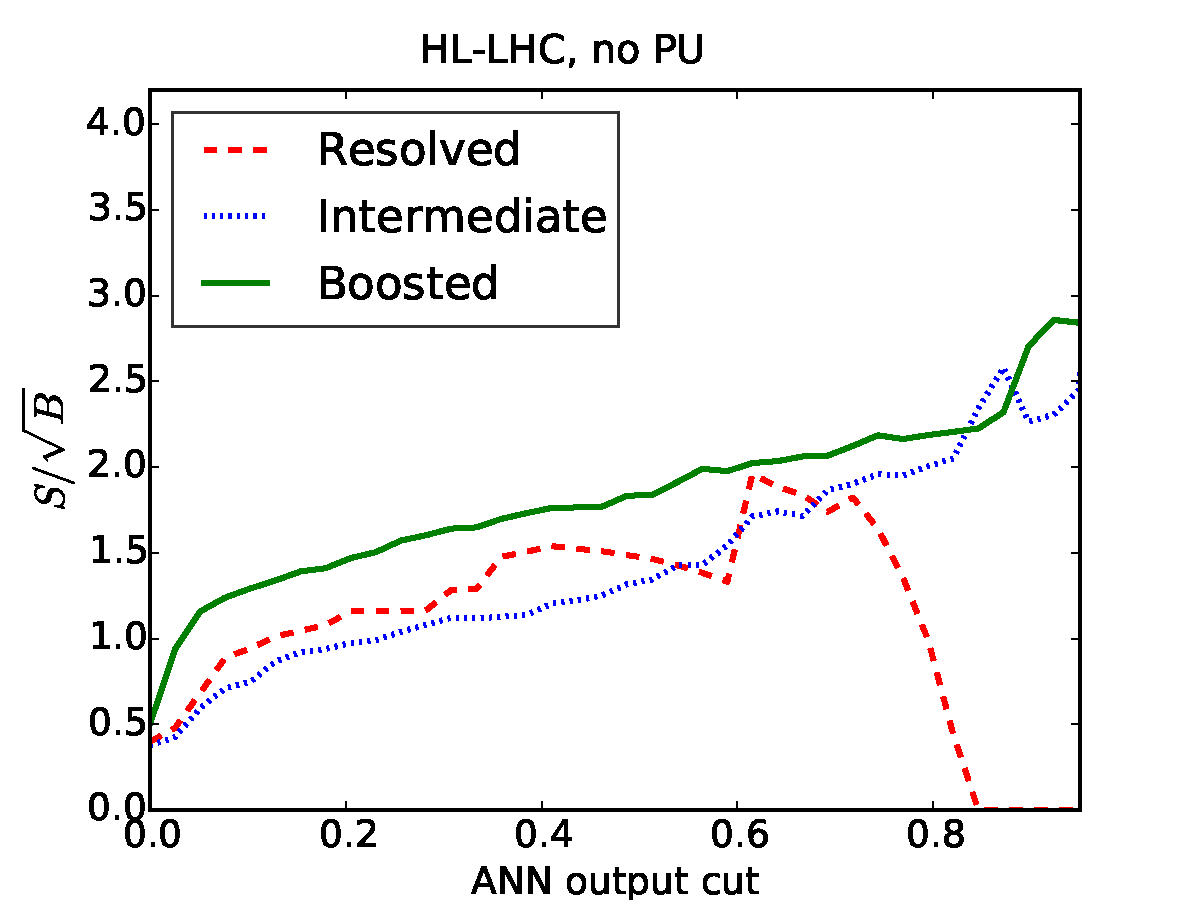
\includegraphics[width=0.48\textwidth]{plots/ssb_noPU.pdf}
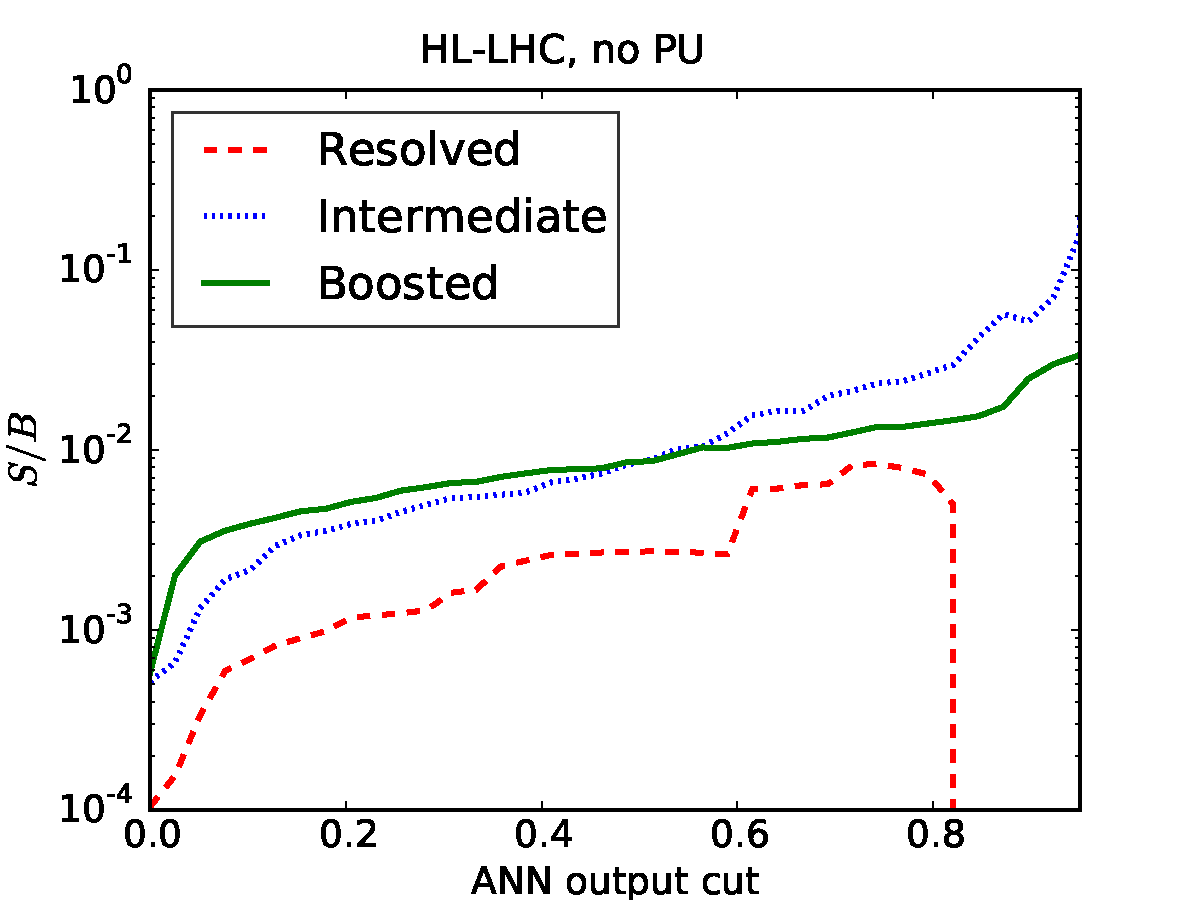
\includegraphics[width=0.48\textwidth]{plots/sb_noPU.pdf}
\caption{\small
  The values of the signal significance, $S/\sqrt{B}$, and of the
  signal over background ratio, $S/B$, for the boosted, intermediate
  and resolved categories as a function of the cut
  $y_{\rm cut}$ in the ANN output.
  %
  The $y_{\rm cut}=0$
  results are those at the end of the cut-based
  analysis. {\bf Update with 100 TeV numbers}
}
\label{fig:sb_mva}
\end{center}
\end{figure}
%%%%%%%%%%%%%%%%%%%%%%%

The results for the signal significance $S/\sqrt{B}$ and
the signal over background ratio
$S/B$ as a function of $y_{\rm cut}$
for the three categories are given in 
Fig.~\ref{fig:sb_mva}.
%
The values 
for $y_{\rm cut}=0$ correspond to those at
the end of the loose cut-based analysis.
%
We observe how in the three
 categories there is a marked  improvement in signal
significance as compared to the pre-MVA results.
%
We also observe a substantial enhancement in $S/B$, arising
from the background suppression achieved by the MVA, reaching
values of 1\%, 6\% and 3.5\% in the resolved,
intermediate and boosted categories.
%
This improvement in $S/B$ is crucial to ensure the feasibility
of this measurement, since it allows systematic
uncertainties in the background determination to
be at most of a similar size.


%%%%%%%%%%%%%%%%%%%%%%%%%%%%%%%%%%%%%%%%%%%%%%%%%%%%%%%%%%%%%%%%%%%%%%%%%%%%
\begin{table}[t]
  \centering
  \begin{tabular}{|c|l|c|c|c|c|}
    \hline
    \multicolumn{6}{|c|}{FCC100, $\mathcal{L}=10$ ab$^{-1}$} \\
    \hline
    \hline
    Category  &   &  $N_{\rm ev}$ signal &  $N_{\rm ev}$ back  &  $S/\sqrt{B}$ & $S/B$ \\ 
    \hline
    \hline
    \multirow{2}{*}{Boosted} &  $y_{\rm cut}=0$  &        &           &          &         \\
    &  $y_{\rm cut}=$ &       &           &          &         \\
    \hline
    \hline
    \multirow{2}{*}{Intermediate} &  $y_{\rm cut}=0$  &        &           &          &         \\
       &  $y_{\rm cut}=$ &       &           &          &         \\
    \hline
    \hline
      \multirow{2}{*}{Resolved} &  $y_{\rm cut}=0$  &         &           &          &         \\
    &  $y_{\rm cut}= $ &        &           &          &         \\
    \hline
      \end{tabular}
  \caption{\small Post-MVA results, for the optimal value of the
    ANN discriminant $y_{\rm cut}$ in the three categories, compared with the
    corresponding
    pre-MVA results ($y_{\rm cut}=0$).
    %
    We quote the number of signal and
    background events expected for $\mathcal{L}=10$ ab$^{-1}$,
    the signal significance $S/\sqrt{B}$ and
    the signal over background ratio $S/B$.
    %
    \label{table:cutflowMVA}
  }
\end{table}
%%%%%%%%%%%%%%%%%%%%%%%%%%%%%%%%%%%%%%%%%%%%%%%%%%%%%%%%%%%%%%%%%%%%%%%%%%%%


From Table~\ref{table:cutflowMVA} we see that
following the application of the MVA, 
the signal significance in the boosted category increases
from 0.5 to 2.7, with $S/B$ increasing from $0.06\%$ to $3\%$.
%
For the intermediate and resolved categories, $S/\sqrt{B}$
increases from 0.4 to 2.3 and 1.9 respectively, with
the signal over background ratio raising from
$0.05\%$ and $0.01\%$ to 4\% and 1\%.
%
Once the MVA training has been completed, it is possible
to estimate, for each value of
the cut in the ANN output $y_{\rm cut}$, how many
signal and background events are expected at the FCC100
assuming a total integrated luminosity of
 $\mathcal{L}=10$ ab$^{-1}$.
%
We also observe that
in the boosted category, for a value $y_{\rm cut}\simeq 0.9$
we end up with around 300 signal events and $10^4$ background
events.
%
Similar results are obtained in the intermediate and resolved
categories: in the former we find 130 ($3\cdot 10^3$) signal (background)
events for $y_{\rm cut}\simeq 0.85$ (0.60), and in the latter
630 ($10^5$) signal (background) events for
$y_{\rm cut}\simeq 0.6$.
%
Combining the three categories, taking into
account all background components, we obtain for
$\mathcal{L}=10$ ab$^{-1}$ an overall signal
significance of $S/\sqrt{B}\simeq 4.0$.
%
This is a substantial improvement over the corresponding
estimator at 14 TeV.

\paragraph{Extracting the Higgs self-coupling.}  The extraction of the trilinear coupling $\lambda$ from the
  corresponding cross-section is complicated by the
  destructive interference
  between diagrams that depend on $\lambda$ and those that do not.
  %
  Therefore, a measurement of the Higgs pair production
  cross-section does not guarantee an accurate enough determination of the trilinear
  coupling $\lambda$.
  %
 Here we provide a first estimate of the accuracy
  in Higgs self-coupling extraction from the $b\bar{b}b\bar{b}$ final state
  that can be achieved 100 TeV hadron collider.
  %
  A robust estimate of the accuracy of this measurement would requires
  a careful study of the impact 
  experimental systematic uncertainties, which is beyond the scope of this contribution.
  %
  Therefore, we will use a number of simplifying assumptions.

  The sensitivity of in the Higgs self-coupling can be estimated by defining a $\chi^2$
  \be
  \label{eq:chi2profile}
  \chi^2(\lambda) = \frac{\lc \sigma(hh,\lambda) - \sigma(hh,\lambda_{\rm SM})
    \rc^2}{\lp \delta_{\rm stat}\sigma\rp^2+\lp \delta_{\rm sys}\sigma\rp^2 } \, ,
  \ee
  where $\lambda$ is the self-coupling, $\lambda_{\rm SM}$ is the SM value, $\sigma(\lambda)$ is the
  post-MVA signal cross-section for a given value of $\lambda$ and $\delta_{\rm stat}\sigma$ and
  $\delta_{\rm sys}\sigma$ are respectively the statistical and systematic uncertainties in the cross-section
  measurement.
  %
  Signal samples for a range of $\lambda$ values have been generated, and have then been processed
  by the same analysis chain, including the MVA, than the SM samples.
  %
  To avoid introducing theoretical biases, the MVA is non-retrained for the $\lambda\ne \lambda_{\rm SM}$ values.
  %
  The 68\% CL range for the extraction of $\lambda$ can then be found by determining the values $\pm \delta\lambda$
  for which the cross-section satisfies
  \be
  \label{eq:condition}
\chi^2(\lambda_{\rm SM}~^{+\delta\lambda}_{-\delta\lambda})=\chi^2(\lambda_{\rm SM})+1 \, .
\ee
The statistical error is given by $1/\sqrt{N_{\rm ev}}$ with $N_{\rm ev}$ is the post-MVA number of events in each analysis
category.
%
We explore different assumptions on the value of the total systematic uncertainty $\delta_{\rm sys}\sigma$.
%
The final result for the accuracy in the trilinear extraction is obtained by combining the separate results
from the three exclusive categories.

In Fig.~\ref{fig:chi2} we show the post-MVA cross-section in the resolved, intermediate
  and boosted categories as a function of the Higgs self-coupling
  $\lambda/\lambda_{\rm SM}$ in units of the SM coupling.
  %
  In the same figure we also show the $\chi^2(\lambda)$ profile, Eq.~(\ref{eq:chi2profile})
  for the three categories, assuming a total systematic uncertainty of
  10\%.
  %
  Imposing the condition Eq.~(\ref{eq:condition}), we obtain that at the 68\% CL we can constrain the
  Higgs trilinear to be ....

%%%%%%%%%%%%%%%%%%%%%%%%
\begin{figure}[t]
\begin{center}
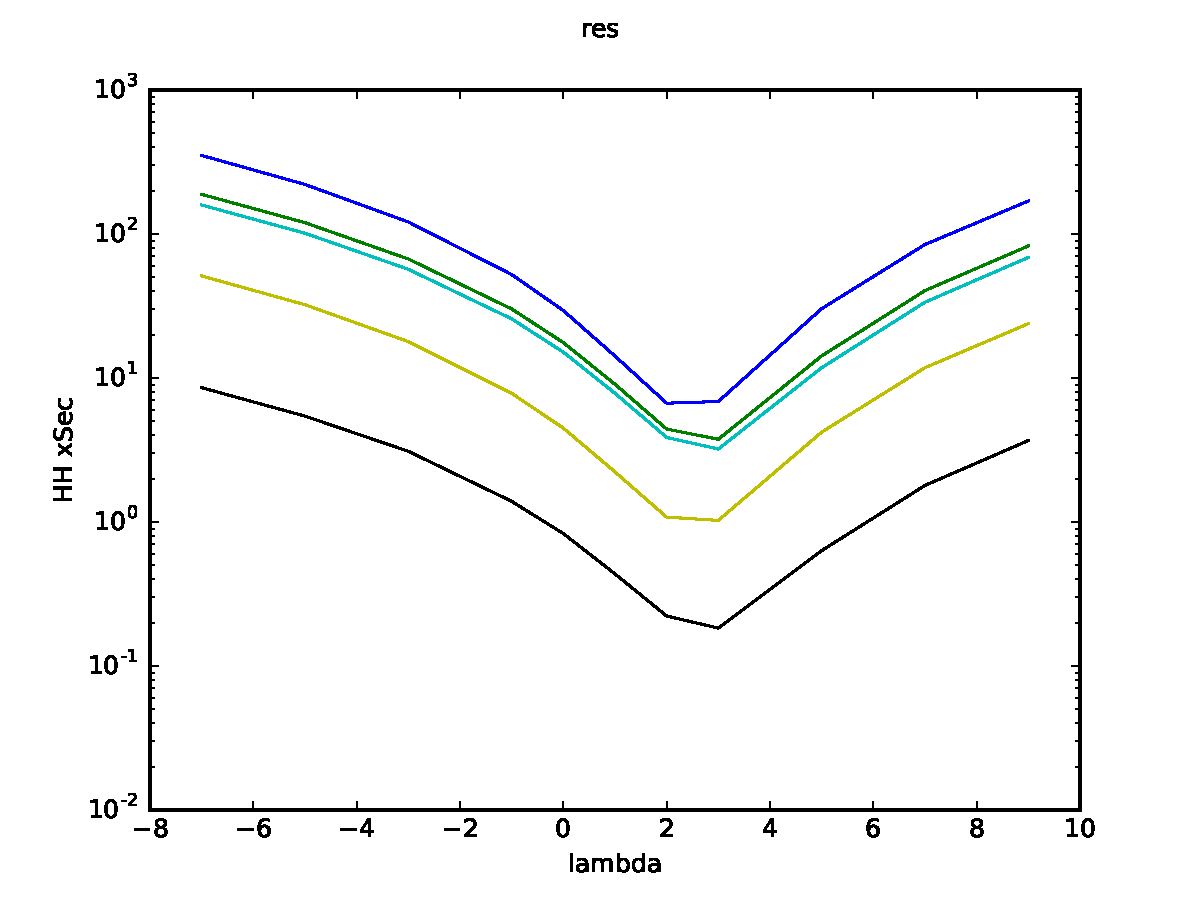
\includegraphics[width=0.48\textwidth]{plots/res.pdf}
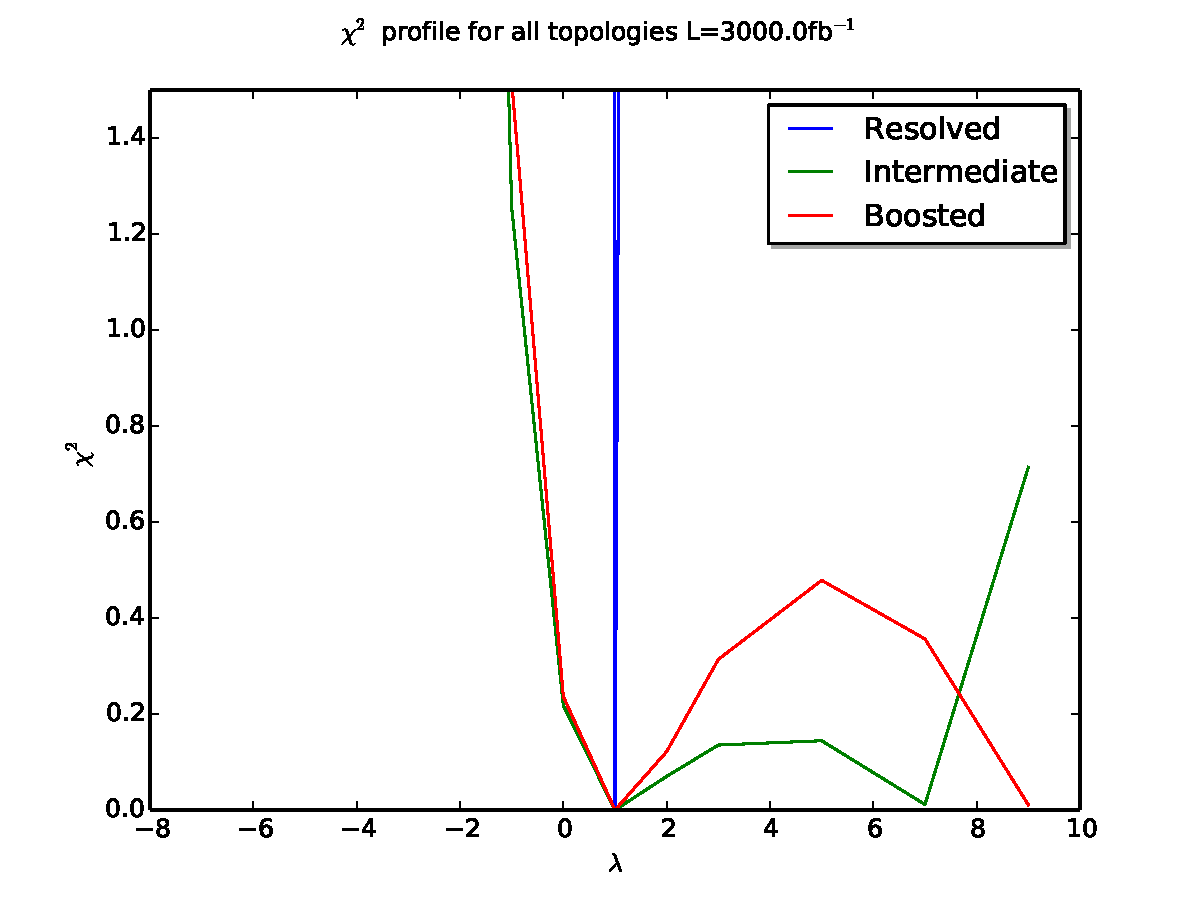
\includegraphics[width=0.48\textwidth]{plots/chi2.pdf}
\caption{\small
  Left plot: the post-MVA cross-section in the resolved, intermediate
  and boosted categories as a function of the Higgs self-coupling
  $\lambda/lambda_{\rm SM}$ in units of the SM coupling.
  %
  Right plot: the $\chi^2(\lambda)$ profile, Eq.~(\ref{eq:chi2profile})
  for the three categories, assuming a total systematic uncertainty of
  10\%.
  {\bf Update}
}
\label{fig:chi2}
\end{center}
\end{figure}
%%%%%%%%%%%%%%%%%%%%%%%
  
\paragraph{Summary.} In this contribution we have performed a first exploration of the accuracy that can be expected
for the extraction of the Higgs self-couplings at a 100 TeV hadron collider using the $b\bar{b}b\bar{b}$ final state. 

%%%%%%%%%%%%%%%%%%

\bibliography{HH4b}



\end{document}
